\documentclass[11pt,a4paper]{article}
\usepackage[a4paper,margin=2cm]{geometry}
\usepackage[T1]{fontenc}\usepackage{times}\usepackage{parskip}
\usepackage{graphicx,booktabs,tabularx,array,xcolor,enumitem}
\usepackage[font=small,labelfont=bf,skip=4pt]{caption}
\usepackage[hidelinks]{hyperref}
\renewcommand{\arraystretch}{1.15}
\newcolumntype{L}[1]{>{\raggedright\arraybackslash}p{#1}}
\newcolumntype{Y}{>{\raggedright\arraybackslash}X}
\definecolor{good}{HTML}{1F6F3A}\definecolor{bad}{HTML}{B3261E}
\setlist{itemsep=1pt,topsep=2pt}
\begin{document}

{\Large\bfseries GeoCrop: Cropland Model Replacement and Comparison}\\[2pt]
{\large Previous Random Forest vs.\ class-weighted LSTM (Gajardo 2023 / Kerner 2020)}\\[2pt]
{\small F26-155-GeoCrop \;|\; AOI~1, Columbia Basin, Washington \;|\; 23 November 2026}

\section*{Summary}
\begin{itemize}
  \item The LSTM is now the cropland model of the platform; the Random Forest (RF) is kept as a disabled backup.
  \item \textbf{On AOI~1} both models agree with CDL~2022 on 93.6\% of pixels. The LSTM has the higher
        \textbf{balanced accuracy (0.942 vs.\ 0.929)} and makes \textbf{3.8$\times$ fewer false cropland} pixels
        (shrubland, wetlands, towns), but misses more real cropland, mostly \textbf{apple orchards and fallow land}.
  \item \textbf{On new areas} (the fair test, from the model team's report) the LSTM scores 0.865 balanced accuracy;
        Random Forests score 0.71--0.72. AOI~1 favours the RF, which was trained on AOI~1 itself.
  \item The LSTM is \textbf{730$\times$ smaller} (98~KB vs.\ 72~MB) and mapped the whole AOI in \textbf{15~s} in the platform.
  \item \textcolor{bad}{\textbf{Issue found:}} the crop-type model (unchanged) drops from 62.5\% to 26.1\% when it is fed
        the 2022 monthly composite instead of its own image; see Section~5.
\end{itemize}

\section{What was compared}
\begin{tabularx}{\textwidth}{L{3.3cm} Y Y}
\toprule
 & \textbf{Previous model (RF, backup)} & \textbf{New model (LSTM, active)}\\
\midrule
Algorithm & Random Forest (scikit-learn) & Class-weighted UnrolledLSTM, 64 units, 23{,}681 parameters (PyTorch)\\
Input per pixel & 7 values from one summer composite (B2 B3 B4 B8 B11 B12 NDVI) & 77 values: 7 months (Apr--Oct 2022) $\times$ 11 (10 bands + NDVI)\\
Trained on & AOI~1 only, random 80/20 pixel split & 8 US areas, 300{,}000 pixels; selected by leave-one-area-out\\
Model file & 72~MB & 0.098~MB\\
\bottomrule
\end{tabularx}

\textbf{Test data.} Both models classified AOI~1 and were scored against the 2022 USDA Cropland Data Layer with
the rule both were trained with (14 CDL classes such as water, developed, forest, shrubland, grassland and wetlands
are non-cropland; all other classes are cropland). Scores use the \textbf{1{,}111{,}982 pixels (100{,}078~ha)} inside the
AOI where CDL and both models have a value. The RF read its own image resampled onto the CDL grid (as in its
training); the LSTM read the 2022 monthly composite built with the model team's \texttt{build\_composite\_stac.py}
(April--October, 142 usable of 195 Sentinel-2 scenes; every pixel has at least 6 clear months).

\section{Results on AOI 1}
\begin{table}[h]
\centering\small
\caption{Scores against CDL 2022 (same 1.11 million pixels)}
\begin{tabular}{lrrr}
\toprule
\textbf{Measure} & \textbf{RF (previous)} & \textbf{LSTM (new)} & \textbf{Better}\\
\midrule
Accuracy & 0.936 & 0.936 & tie\\
Balanced accuracy & 0.929 & \textbf{0.942} & LSTM\\
Cropland precision / recall / F1 & 0.930 / \textbf{0.964} / \textbf{0.947} & \textbf{0.979} / 0.912 / 0.944 & --\\
Non-cropland precision / recall / F1 & \textbf{0.944} / 0.894 / 0.918 & 0.882 / \textbf{0.972} / \textbf{0.925} & --\\
False cropland (pixels) & 47{,}920 & \textbf{12{,}702} & LSTM (3.8$\times$ fewer)\\
Missed cropland (pixels) & \textbf{23{,}735} & 58{,}425 & RF\\
Cropland area (CDL: 59{,}527~ha) & 61{,}703~ha (+3.7\%) & 55{,}412~ha ($-$6.9\%) & RF closer\\
Inference time / peak memory (whole AOI) & 3.2~s / 0.66~GB & 10.9~s / 2.2~GB & RF\\
\bottomrule
\end{tabular}
\end{table}

The models agree on 92.2\% of pixels. Where they disagree (86{,}282 pixels) each is right about half the time
(LSTM 43{,}405, RF 42{,}877). The difference is in \emph{how} they err:
\begin{itemize}
  \item \textbf{RF over-calls cropland}: 46\% of its false cropland is shrubland, 15\% grassland, 13\% wetlands, 24\% developed land.
  \item \textbf{LSTM under-calls some cropland}: 31\% of what it misses is apple orchards, 13\% alfalfa, 9\% winter wheat, 8\% potatoes, 8\% fallow.
\end{itemize}

\begin{table}[h]
\centering\small
\caption{Share of each CDL crop that each model labels cropland (recall), main crops in AOI 1}
\begin{tabular}{lrrr@{\hskip 1.2cm}lrrr}
\toprule
\textbf{Crop} & \textbf{Pixels} & \textbf{RF} & \textbf{LSTM} & \textbf{Crop} & \textbf{Pixels} & \textbf{RF} & \textbf{LSTM}\\
\midrule
Alfalfa & 134{,}530 & 0.980 & 0.945 & Dry Beans & 39{,}231 & 0.992 & 0.966\\
Potatoes & 97{,}561 & 0.985 & 0.951 & Peas & 21{,}232 & 0.964 & 0.944\\
Corn & 93{,}302 & 0.987 & 0.974 & Sod/Grass Seed & 17{,}633 & 0.958 & 0.960\\
Other Hay & 59{,}381 & 0.984 & 0.938 & Onions & 11{,}545 & 0.989 & 0.951\\
Winter Wheat & 55{,}475 & 0.958 & 0.902 & Spring Wheat & 6{,}830 & 0.970 & 0.934\\
Sweet Corn & 46{,}252 & 0.984 & 0.965 & Fallow/Idle & 6{,}003 & 0.470 & \textcolor{bad}{0.223}\\
\textbf{Apples} & 44{,}829 & 0.851 & \textcolor{bad}{\textbf{0.595}} & & & & \\
\bottomrule
\end{tabular}
\end{table}

\begin{figure}[h]
\centering
\begin{tabular}{cccc}
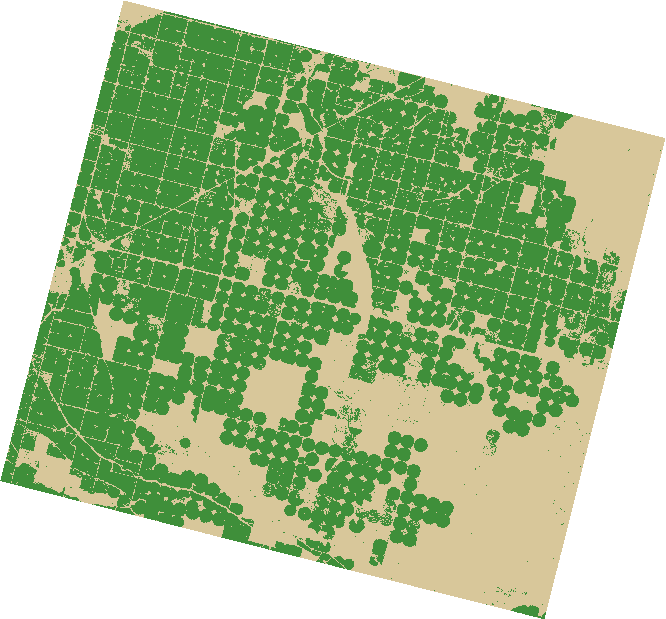
\includegraphics[width=0.225\textwidth]{figures/map_cdl.png} &
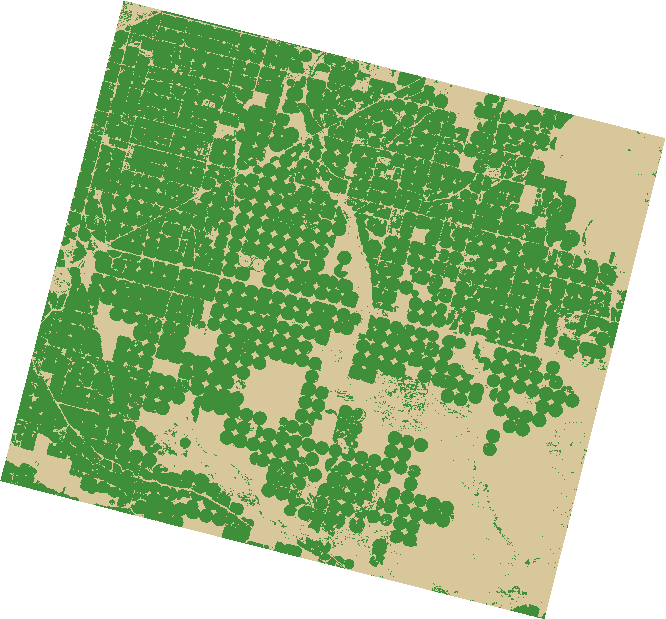
\includegraphics[width=0.225\textwidth]{figures/map_rf.png} &
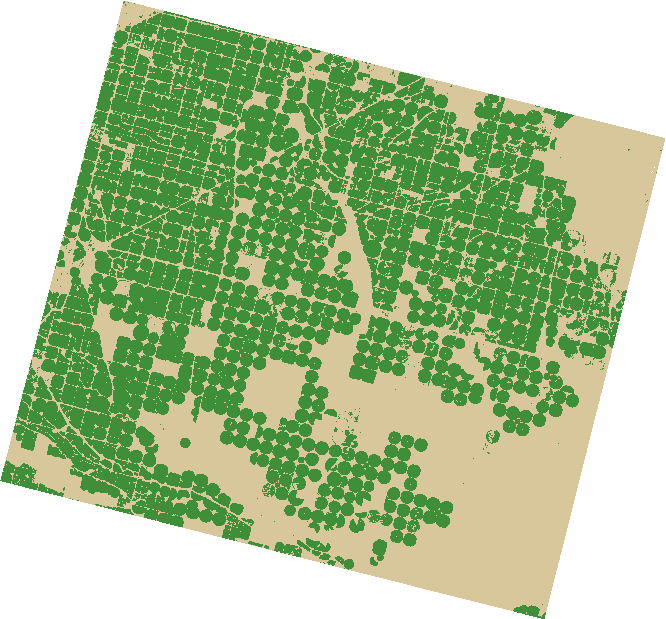
\includegraphics[width=0.225\textwidth]{figures/map_lstm.png} &
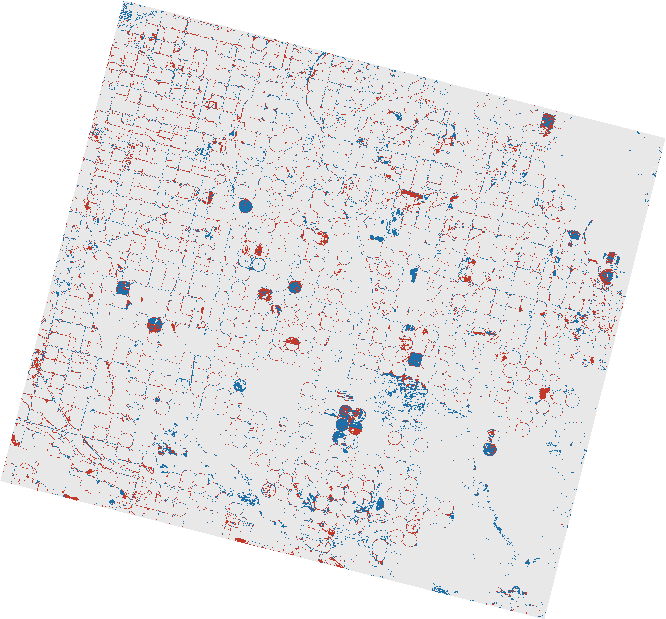
\includegraphics[width=0.225\textwidth]{figures/map_disagreement.png}\\
\small CDL 2022 (reference) & \small RF (previous) & \small LSTM (new) & \small Disagreement
\end{tabular}
\caption{AOI 1. Green = cropland, tan = non-cropland. Disagreement map: grey = models agree,
\textcolor[HTML]{1E6FA8}{blue} = only the LSTM is right, \textcolor[HTML]{C0392B}{red} = only the RF is right.
Disagreements follow field edges, roads and a few whole pivots.}
\end{figure}

\section{How to read these numbers}
\begin{itemize}
  \item \textbf{AOI 1 is not a fair test of generalisation.} The RF was trained on 80\% of AOI~1's pixels from the same
        image, so most test pixels are its own training pixels or their neighbours. The LSTM's final model was also
        trained on a sample of AOI~1 (as one of 8 areas). Both scores are therefore optimistic.
  \item \textbf{The fair test is leave-one-area-out} (model team's report): trained on 7 areas, tested on the 8th.
        There the LSTM scores \textbf{0.865} mean balanced accuracy (worst area 0.677, cropland F1 0.899) and Random
        Forests \textbf{0.71--0.72}. This is the result that matters for new uploads.
  \item The RF also works on the 2022 monthly data when its 7 inputs are derived from it (balanced accuracy 0.913),
        so cropland vs.\ non-cropland is stable across years.
  \item \textbf{Known weakness of the LSTM:} orchards and fallow land (flat seasonal curve, similar to natural vegetation).
        This matches the report's finding that area 4 (most diverse crops) is its weak spot.
\end{itemize}

\section{Crop type on the new input (issue)}
When a 77-band composite is uploaded, the crop-type model (unchanged Random Forest) receives its 7 inputs as the
May--September median of the monthly composite. On AOI~1:
\begin{center}\small
\begin{tabular}{lrr}
\toprule
Crop-type input & Accuracy vs.\ CDL (14 classes) & Agreement with original\\
\midrule
Original single composite (its training image) & 0.625 & --\\
Derived from the 2022 monthly composite & \textcolor{bad}{0.261} & 24\%\\
\bottomrule
\end{tabular}
\end{center}
Brightness levels match (band medians within 1--15\%), but the same fields have weakly related values
(correlation 0.27--0.44). The most likely reason is a \textbf{different year}: the export script of the original
image (\texttt{export\_sentinel2\_gee.py}) uses 2024 dates, while CDL and the new composite are 2022, and crops rotate.
The crop-type model has therefore learned its own image rather than 2022 crops. \textbf{Cropland is not affected.}
Options: (a) retrain this baseline crop-type model on the 2022 monthly composite (minutes); (b) bring in the
monthly-composite LightGBM pipeline from the crop-type evaluation (planned for Iteration~2), which takes this
input natively.

\section{Platform changes}
\begin{tabularx}{\textwidth}{L{4.6cm} Y}
\toprule
\textbf{Change} & \textbf{Effect}\\
\midrule
New plug-in \texttt{cropland} (LSTM) & Model team's code used unchanged; \texttt{model.pt} loaded in safe mode (weights only); identical outputs to their loader.\\
Previous RF as \texttt{cropland\_rf\_legacy} & Disabled backup; existing 23 cropland results relabelled as the previous model. Switch back: swap \texttt{enabled} in the two manifests.\\
Uploads up to 80 bands & 77-band monthly composites accepted; crop type and NDVI derive their inputs automatically.\\
3-band July display copy & Imagery tiles \textbf{43~ms instead of 552~ms} (median, 12 tiles, zoom 12).\\
Integer storage of composites & AOI~1 composite stored as int16 (270~MB with overviews) instead of float32 (about twice the size).\\
AOI~1 composite as a source image & New model can be re-run on AOI~1 from \emph{Analyze $\rightarrow$ Re-analyse an existing image}; full AOI in 15~s.\\
\bottomrule
\end{tabularx}

\textbf{Reproduce:} run \texttt{tools/compare\_cropland\_models.py all} inside the worker container;\\ the raw numbers are in \texttt{comparison.json}.
\end{document}
